\documentclass[10pt]{article}
\usepackage{pictex,amsmath,amssymb,amsbsy,amsfonts,amsthm,verbatim}
\usepackage{graphics}
\usepackage{fullpage}
\usepackage{fancyhdr}
\usepackage{algorithm,algorithmic}
\usepackage{multirow}
\usepackage{graphicx}
\setlength{\voffset}{-0.25in}
\setlength{\headsep}{+0.5in}
\setlength{\parskip}{1em}
\setlength{\parindent}{0em}

\def\vu{\mathbf{u}}
\def\vv{\mathbf{v}}
\def\vs{\mathbf{s}}
\def\vb{\mathbf{b}}
\def\vw{\mathbf{v}}

\renewcommand{\implies}{\rightarrow}
\renewcommand{\lor}{\vee}
\renewcommand{\land}{wedge}
\renewcommand{\iff}{\leffrightarrow}
\newcommand{\xor}{\oplus}
\newcommand{\TRUE}{\mathbf{T}}
\newcommand{\FALSE}{\mathbf{F}}
\newcommand{\universe}{\mathcal{U}}

\usepackage{xcolor}
\usepackage{titlesec}
\usepackage{mdframed}
\usepackage{amsmath}
\usepackage[utf8]{vietnam}

\newmdenv[linecolor=blue,skipabove=\topsep.skipbelow=\topsep,leftmargin=5pt,rightmargin=-5pt,innerleftmargin=5pt,innerrightmargin=5pt]{mybox}

\begin{document}t
\begin{center}
\textbf{\underline{INDEFINITE INTEGRAL}}
\end{center}
\textbf{SOME BASIC FORMULAS OF INDEFINITE INTEGRALS}
\begin{itemize}
	\item $\displaystyle \int \dfrac{dx}{x^2-a^2} = \dfrac{1}{2a}ln|\dfrac{x-a}{x+a}| + C$
	\item $\displaystyle \int \dfrac{dx}{\sqrt{x^2 +a}} = ln|x+ \sqrt{x^2 +a}| + C$
	\item $\displaystyle \int \sqrt{a^2-x^2}dx$.\\
	Let x = asint, where $\dfrac{- \pi}{2} \le t \le \dfrac{\pi}{2}$
\end{itemize}
\textbf{THE SUBSTITUTION RULE }
\begin{mybox}
\begin{center}
$\displaystyle \int f(u(x))du(x)= F(u(x))+C$
\end{center}t
\end{mybox}
\textbf{INTEGRATE BY PARTS}
\begin{mybox}
\begin{center}
$\displaystyle \int udv = uv- \int vdu$
\end{center}
\end{mybox}
\textbf{REDUCTION FORMULA} (Công thức truy hồi)
\begin{mybox}
\begin{center}
$I_{n+1} = \dfrac{1}{2na^2} \times \dfrac{x}{(x^2+a^2)^n} + \dfrac{2n-1}{2na^2} \times I_n$
\end{center}
\end{mybox}
Since:\\
\begin{center}
$I_1= \displaystyle \int \dfrac{dx}{x^2+a^2} = \dfrac{1}{a}arctan \dfrac{x}{a}+C$
\end{center}
When\\
\begin{mybox}
\begin{center}
$I_n = \displaystyle \int \dfrac{dx}{(x^2+a^2)^n} (n \in N)$
\end{center}
\end{mybox}
\textbf{The indefinte integrals of these partial fractions}
\begin{enumerate}
	%1
	\item $\displaystyle \int \dfrac{A}{x-a}dx=Aln|x-a| +C$
	%2
	\item $\displaystyle \int \dfrac{A}{(x-a)^n}dx= \dfrac{A}{(1-n)(x-a)^{n-1}}+C,(n \not = 1)$
	%3
	\item $\displaystyle \int\dfrac{Mx+N}{x^2+px+q}dx= \dfrac{M}{2} \int \dfrac{(2x+p)dx}{x^2+px+q} + (N - \dfrac{Mp}{2}) \int \dfrac{dx}{\displaystyle(x+ \dfrac{p}{2})^2+q- \dfrac{p^2}{4}} = \dfrac{M}{2} ln|x^2+px+q|+(N- \dfrac{Mp}{2}) \times \dfrac{1}{\sqrt{q- \dfrac{p^2}{4}}} arctan \dfrac{x+ \dfrac{p}{2}}{\sqrt{q- \dfrac{p^2}{4}}} +C$
	%4
	\item $ \displaystyle \int \dfrac{Mx+N}{(x^2+px+q)^m}dx = \dfrac{M}{2} \int \dfrac{2x+p}{(x^2+px+q)^m}dx + (N - \dfrac{Mp}{2}) \int \dfrac{dx}{(x^2+px+q)^m}\\
 = \dfrac{M}{2} \times \dfrac{(x^2+px+q)^{-m+1}}{-m+1} + (N- \dfrac{Mp}{2} \int \dfrac{dx}{(x^2+px+q)^m},$\\
	Where:\\
\\
	$\int \dfrac{dx}{(x^2+px+q)^m} = \int \dfrac{dx}{\left[(x+ \dfrac{p}{2})^2 + (q- \dfrac{p^2}{4}\right]^m}$ 
\end{enumerate}
\textbf{INTERATION OF RATIONAL FUNCTIONS}\\
\begin{center}
$I= \displaystyle \int \dfrac{P_n(x)}{Q_m(x)}dx$
\end{center}
\textbf{METHOD OF PARTIAL FRACTIONS}
\begin{enumerate}
	%1
    \item If $n \ge m  \mbox{ then we devide } P_n(x) \mbox{ into } Q_n(x):$\\
\begin{center}
$\dfrac{P_n(x)}{Q_m(x)} = S(x) + \dfrac{R(x)}{Q_m(x)}$
\end{center}    
	%2
	\item If n < m then we factorize the denominator as:\\

	$\dfrac{P_n(x)}{Q_m(x)} = \dfrac{A_1}{x-a} + \dfrac{A_2}{(x-a)^2} + ... + \dfrac{A_k}{(x-a)^k} + ... + \dfrac{M_1x+N_1}{x^2+px+q} + ... + \dfrac{M_lx+N_l}{(x^2+px+q)^l}$
	%3
	\item $\displaystyle \int \dfrac{dx}{(x - \alpha) \sqrt{ax^2+bx+c}}$\\
	\textbf{Solution:} Let $x - \alpha = \dfrac{1}{t}$
	%4
	\item $\displaystyle \int \dfrac{dx}{(x^2-a) \sqrt{ax^2+c}}.$\\
	\textbf{Solution:} Let t = $\displaystyle \sqrt{a+ \dfrac{c}{x^2}}.$
	%5
	\item $ \displaystyle \int R(sinx,cosx)dx$.\\
	\pagebreak
	Let $t = tan \dfrac{x}{2}$. Then:
      $$     
	\begin{cases}
	sinx = \dfrac{2t}{1+t^2}\\

	cosx = \dfrac{1-t^2}{1+t^2}\\

	tanx = \dfrac{2t}{1-t^2}\\

	cotx = \dfrac{1-t^2}{2t}
	\end{cases}
      $$
  \end{enumerate}
\pagebreak
\begin{center}
\textbf{DEFINITE INTEGRAL}
\end{center}
\begin{enumerate}
	%1
	\item \textbf{Newton-Leibniz Formula}\\
	If f(x) is continous on $\left[a,b\right]$, then:
	\begin{mybox}
	\begin{center}
	$\displaystyle \int_{a}^{b}f(x)dx = \int_{a}^{b}F'(x)dx = F(x) |_{a}^{b} = F(a) - F(b)$
	\end{center}
	\end{mybox}
	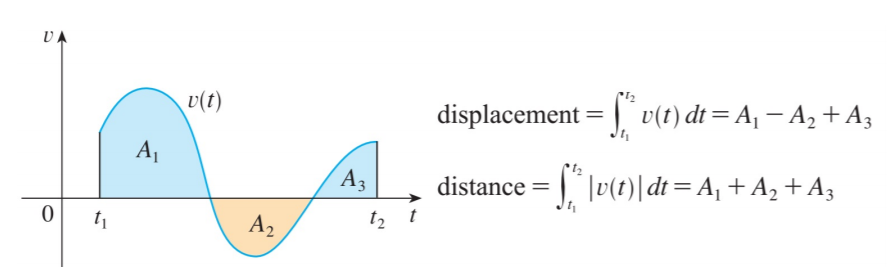
\includegraphics{hinh}
	%2
	\item \textbf{Integration by parts for Definite Integrals}\\
	\begin{mybox}
	\begin{center}
	$\displaystyle \int_{a}^{b}udv = uv|_{a}^{b} - \int_{a}^{b}vdu$
	\end{center}
	\end{mybox}
	%3
	\item \textbf{The Substition Rule for Definite Integrals}
	\begin{mybox}
	\begin{center}
	$\displaystyle \int_{a}^{b}f(u(x)).u'(x)dx = \int_{\alpha}^{\beta}f(t)dt$
	\end{center}
	\end{mybox}
	For $\alpha = u(a) ; \beta = u(b)$
	%4
	\item \textbf{Integral of Symmertric Functions}
	\begin{itemize}
		\item If f(x) is \textit{\textbf{odd funtion}}:
		\begin{mybox}
		\begin{center}
		$\displaystyle \int_{-a}^{a}f(x)dx = 0$
		\end{center}
		\end{mybox}
		\item If f(x) is \textit{\textbf{even function}}:
		\begin{mybox}
		\begin{center}
		$\displaystyle \int_{-a}^{a}f(x)dx = 2 \int_{0}^{a}f(x)dx$
		\end{center}
		\end{mybox}
	\end{itemize}
\end{enumerate}
\pagebreak
\begin{center}
\textbf{Aplication of Definite Integral}
\end{center}
\begin{enumerate}
	%1
	\item \textbf{Area}\\
	The \textbf{area} between the curves \textbf{y = f(x)} and \textbf{y = g(x)} and between \textbf{x = a and x = b} is:
	\begin{mybox}
	\begin{center}
	$A = \displaystyle \int_{a}^{b} |f(x) - g(x)|dx$
	\end{center}
	\end{mybox}
	%2
	\item \textbf{The volume of the solid in x-axis}
	\begin{mybox}
	\begin{center}
	$V_x = \pi \displaystyle \int_{a}^{b}f^2(x)dx$
	\end{center}
	\end{mybox}
	%3
	\item \textbf{The volume of the solid in y-axis}
	\begin{mybox}
	\begin{center}
	$V_y = \pi \displaystyle \int_{a}^{b}g^2ydy$
	\end{center}
	\end{mybox}
	%4
	\item \textbf{The Arc Length Formula}
	\begin{mybox}
	\begin{center}
	$L = \displaystyle \int_{a}^{b} \sqrt{1 + f'(x)^2}dx$
	\end{center}
	\end{mybox}
	%5
	\item \textbf{Surface Area}
	\begin{mybox}
	\begin{center}
	$S = 2 \pi \displaystyle \int_{a}^{b} f(x) \sqrt{1 + f'(x)^2}dx$
	\end{center}
	\end{mybox}
\end{enumerate} 
\end{document}	